% (c) 2015 Daniele Zambelli daniele.zambelli@gmail.com

\chapter{La parabola nel piano cartesiano}

\section{Rappresentazione del trinomio di secondo grado}
\label{sec:parabola_rappresentazionetrinomio}

Dopo aver studiato le equazioni di primo grado abbiamo studiato il 
comportamento dei polinomi di primo grado e abbiamo visto che si possono 
collegare con le rette nel piano cartesiano. Vediamo ora cosa succede con i
polinomi di secondo grado. Partiamo da un esempio, consideriamo il polinomio: 
$P(x)=x^2 -2x -3$ chiamiamo $y$ il valore che assume il polinomio quando diamo 
a $x$ diversi valori. Per iniziare a $x$ diamo dei valori interi ottenendo così 
una successione di numeri che riportiamo in una tabella:

\begin{figure}[h]
 \centering
 \begin{minipage}[]{.48\textwidth}
  \begin{center}
   \begin{tabular}{r|l}
    $x$   & $y=x^2-2x-2$ \\
    \hline
    \dots & \dots \\
    $-5$ & $(-5)^2 -2(-5) -3 = 33$ \\
    $-4$ & $(-4)^2 -2(-4) -3 = 22$ \\
    $-3$ & $(-3)^2 -2(-3) -3 = 13$ \\
    $-2$ & $(-2)^2 -2(-2) -3 = 6$ \\
    $-1$ & $(-1)^2 -2(-1) -3 = 1$ \\
     $0$ & $(0)^2 -2(0) -3 = -2$ \\
    $+1$ & $(+1)^2 -2(+1) -3 = -3$ \\
    $+2$ & $(+2)^2 -2(+2) -3 = -2$ \\
    $+3$ & $(+3)^2 -2(+3) -3 = 1$ \\
    $+4$ & $(+4)^2 -2(+4) -3 = 6$ \\
    $+5$ & $(+5)^2 -2(+5) -3 = 13$ \\
    \dots & \dots \\
   \end{tabular}
  \caption{Alcuni valori del trinomio...} \label{tab:trinomio0}
  \end{center}
 \end{minipage}
\begin{minipage}[]{.48\textwidth}
\begin{center}
\begin{inaccessibleblock}[I punti della tabella precedente riportati nel piano 
cartesiano si dispongono lungo una curva.]
  % (c) 2014 Daniele Zambelli - daniele.zambelli@gmail.com

%%%
% Alcuni punti di una parabola.
%%

\disegno{
\rcom{-5}{+5}{-4}{13}{gray!50, very thin, step=1}
\foreach \pi in {
% (-4, 22), 
(-3, 13), (-2, 6), (-1, 1), 
(0, -2), (1, -3), (2, -2), (3, 1), (4, 6), (5, 13)}
 \filldraw [Maroon!50!black] \pi circle (1.5pt);
}

  \caption{...i corrispondenti punti.} \label{fig:trinomio0}
\end{inaccessibleblock}
\end{center}
\end{minipage}
\end{figure}

% \vspace{5mm}
Osservando la disposizione dei punti possiamo porci alcune domande:
\begin{enumerate*}
 \item A ogni valore di $x$ corrisponde un ben preciso valore di $y$?
 \item Tutti i valori di $y$ sono immagine di un qualche valore di $x$?
 \item C'è qualche valore di $y$ che è immagine di più valori di $x$?.
 \item I punti ottenuti non sono allineati, si può riconoscere una forma 
  particolare?.
 \item Possiamo individuare un punto particolare.
 \item Possiamo riconoscere una simmetria?.
 \item Cosa possiamo pensare che succeda quando $x$ diventa sempre più piccolo?
 \item E quando $x$ diventa sempre più grande?
\end{enumerate*}

Possiamo osservare che:
\begin{enumerate*}
 \item Per ogni valore di $x$ troviamo un unico valore di $y$, infatti 
  le operazioni presenti nel polinomio (addizione, moltiplicazione, potenza) 
  danno tutte un solo risultato. Il polinomio definisce una \emph{funzione}
  che mette in relazione numeri reali con numeri reali.
 \item Alcuni valori di $y$ non corrispondono a nessun valore di $x$. 
  La funzione non è \emph{suriettiva}.
 \item Alcuni valori di $y$ corrispondono a due diversi valori di $x$.
  La funzione non è \emph{iniettiva}.
 \item I punti non sono allineati, suggerendo una figura con 
 la concavità verso l'alto.
 \item I punti scendono fino ad un valore minimo, il punto più in basso si 
  chiama \emph{vertice}.
 \item C'è una simmetria nella disposizione dei punti, infatti allontanandosi 
  vero destra o sinistra dal vertice della stessa quantità si arriva sempre 
  alla stessa altezza.
 \item Più piccolo diventa $x$, andando verso $-infty$, più grande diventa il 
  valore del polinomio e cresce sempre più in fretta. 
  Questo è dovuto al fatto che $x^2$ è sempre positivo.
 \item Più grande diventa $x$, andando verso $+infty$, più grande diventa il 
  valore del polinomio e cresce sempre più in fretta. 
  Anche questo dipende da $x^2$ è sempre positivo.
\end{enumerate*}

Ma noi siamo interessati a sapere il valore del polinomio per qualunque valore 
che diamo alla variabile $x$, non solo per valori interi. Costruiamo una nuova 
tabella aggiungendo anche alcuni nuovi valori. Questa volta, per i calcoli 
utilizziamo la calcolatrice.

\begin{figure}[h]
 \begin{minipage}[]{.48\textwidth}
  \begin{center}
   \begin{tabular}{r|l}
    $x$   & $y=x^2-2x-2$ \\
    \hline
    \dots & \dots \\
%     $-5,0$ & $(-5)^2 -2(-5) -3 = 33$ \\
    $-4,5$ & $(-4,5)^2 -2(-4,5) -3 = 27,25$ \\
%     $-4,0$ & $(-4)^2 -2(-4) -3 = 22$ \\
    $-3,5$ & $(-3,5)^2 -2(-3,5) -3 = 17,25$ \\
%     $-3,0$ & $(-3)^2 -2(-3) -3 = 13$ \\
    $-2,5$ & $(-2,5)^2 -2(-2,5) -3 = 9,25$ \\
%     $-2,0$ & $(-2)^2 -2(-2) -3 = 6$ \\
    $-1,5$ & $(-1,5)^2 -2(-1,5) -3 = 3,25$ \\
%     $-1,0$ & $(-1)^2 -2(-1) -3 = 1$ \\
    $-0,5$ & $(0,5)^2 -2(0,5) -3 = -0,75$ \\
%      $0,0$ & $(0)^2 -2(0) -3 = -2$ \\
    $+0,5$ & $(0,5)^2 -2(0,5) -3 = -2,75$ \\
%     $+1,0$ & $(+1)^2 -2(+1) -3 = -3$ \\
    $+1,5$ & $(+1,5)^2 -2(+1,5) -3 = -2,75$ \\
%     $+2,0$ & $(+2)^2 -2(+2) -3 = -2$ \\
    $+2,5$ & $(+2,5)^2 -2(+2,5) -3 = -0,75$ \\
%     $+3,0$ & $(+3)^2 -2(+3) -3 = 1$ \\
    $+3,5$ & $(+3,5)^2 -2(+3,5) -3 = 3,25$ \\
%     $+4,0$ & $(+4)^2 -2(+4) -3 = 6$ \\
    $+4,5$ & $(+4,5)^2 -2(+4,5) -3 = 9,25$ \\
%     $+5,0$ & $(+5)^2 -2(+5) -3 = 13$ \\
    $+5,5,0$ & $(+5,5)^2 -2(+5,5) -3 = 17,25$ \\
    \dots & \dots \\
   \end{tabular}
  \caption{Alcuni valori del trinomio...} \label{tab:tabella1}
  \end{center}
\end{minipage}
\begin{minipage}[]{.48\textwidth}
\begin{center}
\begin{inaccessibleblock}[I punti della tabella precedente riportati nel piano 
cartesiano si dispongono lungo una curva.]
 % (c) 2014 Daniele Zambelli - daniele.zambelli@gmail.com

%%%
% Varie prove per il disegno di una parabola nel piano cartesiano.
%%%%
%  
\begin{tikzpicture}[x=5mm, y=5mm, smooth]

\tkzInit[xmin=-10.5,xmax=+10.5,ymin=-10.5,ymax=+15.5]

\clip (-5.3, -4.3) rectangle (5.7, 13.8);

% (c) 2014 Daniele Zambelli - daniele.zambelli@gmail.com

%%%
% Piano cartesiano: da (-10; -10) a (+5; +10)
%%%%

% Griglia
\draw[gray!50, very thin, step=1] (-10.2, -10.2) grid (5.2, 13.2);

%Asse x
\draw [-{Stealth[length=2mm, open, round]}] (-10.3,0) -- (5.5,0) node [below]
      {$x$};

%Asse y
\draw [-{Stealth[length=2mm, open, round]}] (0, -10.3) -- (0, 13.5) node [left]  
      {$y$};


\foreach \pi in {
(-4, 22), (-3, 13), (-2, 6), (-1, 1), 
(0, -2), (1, -3), (2, -2), (3, 1), 
(4, 6), (5, 13),
(-4.5, 27.25), (-3.5, 17.25), (-2.5, 9.25), (-1.5, 3.25), 
(-0.5, -0.75), (0.5, -2.75), (1.5, -2.75), (2.5, -0.75), (3.5, 3.25), 
(4.5, 9.25), (5, 17.25)}
 \filldraw [Maroon!50!black] \pi circle (1.5pt);


% \tkzFct[domain=-5:+5, ultra thick, color=Maroon!50!black]{x*x+x-1}
\end{tikzpicture}

 \caption{...i corrispondenti punti.}\label{fig:trinomio1}
\end{inaccessibleblock}
\end{center}
\end{minipage}
\end{figure}

Possiamo osservare che:

\begin{enumerate*}
 \item I nuovi punti confermano le considerazioni che avevamo fatto riguardo 
 alla simmetria della figura.
 \item Se prendiamo un valore di $x$ compreso tra altri due valori, anche il 
 corrispondente valore di $y$ sarà compreso tra i due valori di y 
 corrispondenti:~$x_0 < x <_1 \Rightarrow P(x_0) < P(x) < P(x_1)$.
\end{enumerate*}

Se continuiamo ad aggiungere punti otteniamo una linea continua a cui viene 
dato il nome di \emph{parabola}.

\begin{minipage}{.40\textwidth}
\begin{center}
 \begin{inaccessibleblock}[Parabola disegnata nel piano cartesiano.]
%  \begin{wrapfigure}{l}{0pt}
   % (c) 2014 Daniele Zambelli - daniele.zambelli@gmail.com

%%%
% Grafico di un trinomio di secondo grado.
%%

\disegno{
\rcom{-5}{+5}{-4}{13}{gray!50, very thin, step=1}
\tkzInit[xmin=-5.3,xmax=+5.3,ymin=-4.3,ymax=+13.3]
\tkzFct[domain=-5:+6, ultra thick, color=Maroon!50!black]{x*x-2*x-2}
}

  
  \emph{Parabola~$y=x^2-2x-2$}\label{fig:parabola_trinomio2}
% \end{wrapfigure}
\end{inaccessibleblock}
\end{center}
\end{minipage}
\begin{minipage}{.55\textwidth}
Dov'è che la parabola interseca gli assi?

Per quanto riguarda l'asse $y$ è facile, essendo l'equazione 
dell'asse~$y$:~$x=0$,
l'intersezione è la soluzione del sistema:
\[\left\{\begin{array}{l}
 x=0 \\
 y=x^2-2x-2 
\end{array}\right.\]
Il termine di grado zero del polinomio indica il punto in cui la curva 
interseca l'asse $y$. 

Per trovare le intersezioni con l'asse $x$ dobbiamo risolvere il sistema:
\[\left\{\begin{array}{l}
 y=0 \\
 y=x^2-2x-2 
\end{array}\right.\]

che dà come equazione risolutiva l'equazione di secondo grado:
\[x^2-2x-2=0\]

la cui soluzione è:
\[x_{1, 2} = \frac{-b \mp\sqrt{b^2-4ac}}{2a}=
             \frac{+1 \mp\sqrt{1+2}}{1}=+1 \mp\sqrt{3}\]

\end{minipage}


\section{Significato geometrico dei coefficienti}
\label{sec:parabola_coefficienti}

Visto che per disegnare una parabola dobbiamo fare molti calcoli, utilizziamo 
il foglio di calcolo (le seguenti indicazioni riguardano Calc che è il foglio
di calcolo di LibreOffice).

\begin{procedura}
 Per far disegnare parabole ad un foglio di calcolo.
 \begin{enumerate*}
  \item Crea un nuovo foglio di calcolo e salvalo con il 
   nome~``pcoefficientiparabola''.
  \item Intestazioni varie:
   \subitem <A1>: Coefficienti della parabola
   \subitem <D1>: <menu-Inserisci-Oggetto-Formula...> ax\^{}2+bx+c
   \subitem <A3>: a
   \subitem <A3>: <Clic destro - Inserisci commento> Coefficiente termine di 
    secondo grado.
   \subitem <A4>: b
   \subitem <A4>: <Clic destro - Inserisci commento> Coefficiente termine di 
    primo grado.
   \subitem <A5>: c
   \subitem <A5>: <Clic destro - Inserisci commento> Coefficiente termine di 
    grado zero.
   \subitem <A7>: x
   \subitem <b7>: y
  \item Dati
   \subitem <B3>: -0,5
   \subitem <B4>: 1
   \subitem <B3>: 1
   \subitem <A8>: -10
   \subitem <A9>: -9,5
   \subitem seleziona <A8:A9>: una cifra decimale, 
    copia verso il basso fino a <A48>
   \subitem <B8>: =B\$3*A8\^2+B\$4*A8+B\$5 (attento ai simboli \$ che indicano i
    riferimenti assoluti)
   \subitem <B8>: 3 cifre decimali, copia verso il basso fino ad <b48>
  \item Grafico
   \subitem seleziona <A8:B48>
   \subitem <menu-Inserisci-Grafico>
   \subitem XY (Dispersione), Tipo linea: Liscia, Solo linee.
   \subitem Titolo: Parabola nel piano cartesiano
   \subitem Togli la spunta a: Mostra legenda.
   \subitem Metti la spunta a Mostra griglie Asse X e Asse Y.
   \subitem Doppio clic su un numero dell'asse y: 
    <Scala> Minimo -10, Massimo 10, Intervallo principale 1;
    <Linea> Colore Nero;
    <Didascalia> togli la spunta a <Mostra didascalia>.
   \subitem Doppio clic su un numero dell'asse x: 
    <Scala> Minimo -10, Massimo 10, Intervallo principale 1;
    <Linea> Colore Nero;
    <Didascalia> togli la spunta a <Mostra didascalia>.
   \subitem Clicca fuori dal grafico, clicca sul grafico, modifica le 
    dimensioni (``maniglie'' verdi) in modo che i riquadri della griglia 
    siano quadrati.
 \end{enumerate*}
\end{procedura}

Ora Trova i coefficienti che producono le seguenti parabole.

\begin{figure}[h]
\begin{minipage}{.69\textwidth}
 \begin{inaccessibleblock}[Parabola disegnata nel piano cartesiano.]
  % (c) 2014 Daniele Zambelli - daniele.zambelli@gmail.com

%%%
% Varie prove per il disegno di una parabola nel piano cartesiano.
%%%%
%  
\begin{tikzpicture}[x=5mm, y=5mm, smooth]

\tkzInit[xmin=-10.5,xmax=+10.5,ymin=-10.5,ymax=+15.5]

\clip (-10.3, -10.3) rectangle (10.7, 10.7);

% (c) 2014 Daniele Zambelli - daniele.zambelli@gmail.com

%%%
% Piano cartesiano: da (-10; -10) a (+10; +10)
%%%%

% Griglia
\draw[gray!50, very thin, step=1] (-10.2, -10.2) grid (10.2, 10.2);

%Asse x
\draw [-{Stealth[length=2mm, open, round]}] (-10.3,0) -- (10.5,0) node [below]  {$x$};

%Asse y
\draw [-{Stealth[length=2mm, open, round]}] (0, -10.3) -- (0, 10.5) node [left]  {$y$};


\tkzFct[domain=-10:+10, ultra thick, color=Maroon!50!black]{2*x*x+x+2}
% \tkzFct[domain=-10:+10, ultra thick, color=Maroon!50!black]{x*x+x+2}
\tkzFct[domain=-10:+10, ultra thick, color=Maroon!50!black]{0.5*x*x+x+2}
\tkzFct[domain=-10:+10, ultra thick, color=Maroon!50!black]{0.1*x*x+x+2}
\tkzFct[domain=-10:+10, ultra thick, color=Maroon!50!black]{0.01*x*x+x+2}
\tkzFct[domain=-10:+10, ultra thick, color=Green!50!black]{-0.01*x*x+x+2}
\tkzFct[domain=-10:+10, ultra thick, color=Green!50!black]{-0.1*x*x+x+2}
\tkzFct[domain=-10:+10, ultra thick, color=Green!50!black]{-0.5*x*x+x+2}
% \tkzFct[domain=-10:+10, ultra thick, color=Green!50!black]{-x*x+x+2}
\tkzFct[domain=-10:+10, ultra thick, color=Green!50!black]{-2*x*x+x+2}
\node [black] at (-1.5, 9.5) {a};
\node [black] at (-4, 8.5) {b};
\node [black] at (-9, 2) {c};
\node [black] at (-9, -5.5) {d};
\node [black] at (-8, -7.5) {e};
\node [black] at (-5.6, -8.5) {f};
\node [black] at (-3.5, -9.5) {g};
\node [black] at (-1.5, -9.5) {h};
\end{tikzpicture}

  \caption{Parabole con diverse ampiezze} \label{fig:parabola_coeff_a}
\end{inaccessibleblock}
\end{minipage}
\begin{minipage}{.29\textwidth}
 \begin{enumerate}[label=\alph*]
   \item :~$y=...$
   \item :~$y=...$
   \item :~$y=...$
   \item :~$y=...$
   \item :~$y=...$
   \item :~$y=...$
   \item :~$y=...$
   \item :~$y=...$
 \end{enumerate}
\end{minipage}
\end{figure}

\begin{enumerate*}
 \item Se $a>0$ la concavità della parabola è verso l'alto.
 \item Se $a<0$ la concavità della parabola è verso il basso.
 \item Se $a=0$ la parabola non ha concavità, è una retta.
 \item Se il valore assoluto di $a$ è grande la parabola è molto stretta.
 \item Se il valore assoluto di $a$ è vicino a zero la parabola è molto ampia.
 \item Se il valore assoluto di $a$ si avvicina a zero la curva si avvicina a 
  una retta.
\end{enumerate*}

In questi esempi ci sono due coefficienti dell'equazione che non variano, 
quali sono le caratteristiche geometriche comuni a tutte le parabole?

Prova a mantenere costante il coefficiente del termine di secondo grado e 
il coefficiente del termine di primo grado e modifica
il termine noto, 
cosa rimane costante e cosa cambia nelle parabole che ottieni?

Prova a mantenere costante il coefficiente del termine di secondo grado e 
il termine noto e modifica
il coefficiente del termine di primo grado
cosa rimane costante e cosa cambia nelle parabole che ottieni?

In conclusione data l'equazione $y=ax^2+bx+c$ puoi osservare che:
\begin{enumerate*}
 \item $a$ è legato alla concavità della parabola;
 \item $b$ è legato alla pendenza che ha la parabola nel punto in cui 
  interseca l'asse $y$;
 \item $c$ è legato al punto in cui la parabola interseca l'asse $y$.
\end{enumerate*}


\section{Tracciare parabole}
\label{sec:parabola_disegno}

Per disegnare una parabola possiamo completare una tabella calcolando 
abbastanza punti per guidare il disegno di una parabola, come abbiamo fatto
nel primo esempio.
Possiamo anche trovare alcuni punti particolari della parabola:

\begin{enumerate*}
 \item L'intersezione con l'asse $y$: $(0;~c)$.
 \item Le intersezioni con l'asse $x$: si ottengono risolvendo l'equazione
  $ax^2+bx+c=0$.
 \item L'ascissa del vertice, è il punto medio delle intersezioni con 
  l'asse~$x$ e con qualche calcolo si può vedere che è uguale 
  a~$x_V=-\frac{b}{2a}$
 \item L'ordinata del vertice si ottiene sostituendo nell'equazione della 
  parabola $x$ con $x_V$ trovato nel punto precedente: $y_V=x_V^2+bx_V+c$.
\end{enumerate*}

Ogni volta che dobbiamo disegnare una parabola ricordiamoci di trovare almeno
questi~4 elementi. Però ci sono delle parabole che possono essere disegnate 
senza fare tanti calcoli. Per trovare un modo rapido per disegnare le parabole 
Consideriamo innanzitutto la successione dei numeri quadrati.

 \begin{inaccessibleblock}[I primi numeri quadrati rappresentati da 
  schieramenti di punti con evidenziato lo gnomone. La successione dei numeri 
  quadrati e le differenze tra un quadrato e il precedente.]
\begin{figure}
  % (c) 2014 Daniele Zambelli - daniele.zambelli@gmail.com

%%%
% Varie prove per il disegno di una parabola nel piano cartesiano.
%%%%

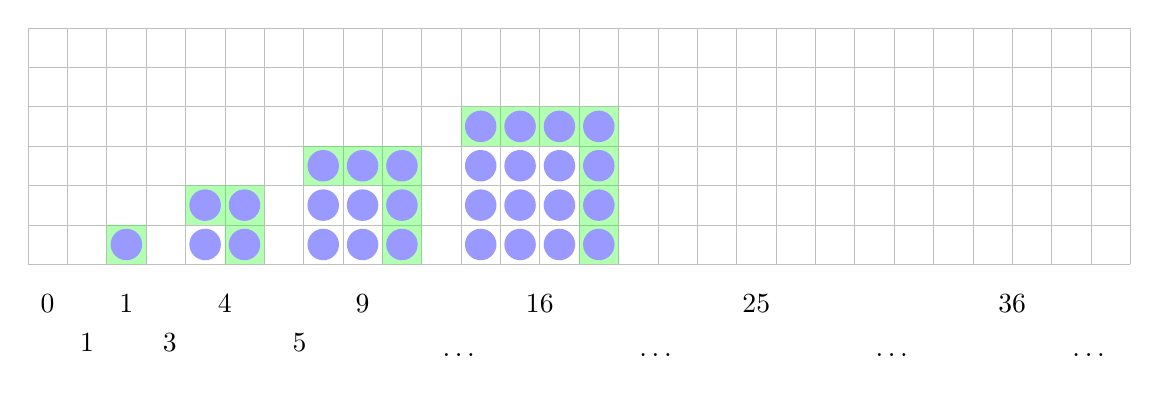
\begin{tikzpicture}[x=5mm, y=5mm, smooth]

\draw[gray!50, very thin, step=1] (-1, 1) grid (27, 7); % Griglia
\draw (-.5, 0) node{0};
\foreach \n in {1, ..., 4} {
    \pgfmathparse{\n * \n / 2 + \n * 3 / 2}
    \xdef\corner{\pgfmathresult}
    \fill[fill=green,fill opacity=0.3] (\corner, \n + 1) --
                                           (\corner - \n, \n + 1) --
                                           (\corner - \n, \n) --
                                           (\corner - 1, \n) --
                                           (\corner - 1, 1) --
                                           (\corner, 1) -- cycle; 
    \foreach \j in {1, ..., \n} {
        \foreach \i in {1, ..., \n} { 
            \fill[blue!40!white] (\n * \n / 2 + \n / 2 -.5 + \i, \j+.5) 
                                   circle (.4);
        }
    }
}
\foreach \n in {1, ..., 6} {
    \pgfmathparse{int(\n * \n)}
    \xdef\square{\pgfmathresult}
    \draw (\n * \n / 2 + \n  , 0) node{\square};
}
\draw (.5  , -1) node{1};
\draw (2.6  , -1) node{3};
\draw (5.9  , -1) node{5};
\draw (10  , -1.3) node{\ldots};
\draw (15  , -1.3) node{\ldots};
\draw (21  , -1.3) node{\ldots};
\draw (26  , -1.3) node{\ldots};

% \clip (-1, -2) rectangle (10, 7);

\end{tikzpicture}

  \caption{I primi numeri quadrati con evidenziato lo gnomone.}
  \label{fig:parabola_quadrati}
\end{figure}
\end{inaccessibleblock}

Possiamo costruire una tabella con la successione dei numeri quadrati e con 
le differenze prime:

\begin{center}
  \begin{tabular}{c c c c c c c c c c}
   $x$        & 0 & 1 & 2 & 3 & 4 & 5 & 6 & 7 & 8 \\
   \hline
   $y=x^2$    & 0 & 1 & 4 & 9 & 16 & 25 & 36 & \ldots & \ldots \\
   \hline
   $\Delta y$ &  & 1 & 3 & 5 & 7 & 9 & 11 & \ldots & \ldots \\
  \end{tabular}
\end{center}
L'ultima riga della tabella presenta una successione nota: la successione dei 
numeri dispari. Guardando la figura \ref{fig:parabola_quadrati} si vede che 
l'ennesimo gnomone è uguale a~$2n+1$. 

Teniamo presente questa successione e proviamo a disegnare la parabola $y=x^2$.
L'ascissa del vertice della parabola è $-\frac{b}{2}=0$ e l'ordinata è 
$y=x_V^2=0^2=0$ disegniamo il vertice nel punto $(0;~0)$. Ogni volta che $x$ 
si allontana dal vertice di~$1$, $y$ aumenta di un numero dispari. 

Riportiamo questi punti nel piano cartesiano e uniamoli con una curva il più 
possibile regolare vedi fig \ref{fig:parabola_parabola0}

% \newpage

\begin{figure}[p]
\begin{minipage}{.50\textwidth}
Andando verso destra:
 \begin{itemize*}
 \item partendo dal vertice che è~$(0;~0)$
 \item $x$ aumenta di~1, $y$ aumenta si~$1$;
 \item $x$ aumenta di~1, $y$ aumenta si~$3$;
 \item $x$ aumenta di~1, $y$ aumenta si~$5$;
 \item \dots
\end{itemize*}
Andando verso sinistra:
\begin{itemize*}
 \item partendo dal vertice che è~$(0;~0)$
 \item $x$ diminuisce di~1, $y$ aumenta si~$1$;
 \item $x$ diminuisce di~1, $y$ aumenta si~$3$;
 \item $x$ diminuisce di~1, $y$ aumenta si~$5$;
 \item \dots
\end{itemize*}
\end{minipage}
\begin{minipage}{.50\textwidth}
\begin{inaccessibleblock}[Parabola di equazione $y=x^2$.]
\centering
  % (c) 2014 Daniele Zambelli - daniele.zambelli@gmail.com

%%%
% Varie prove per il disegno di una parabola nel piano cartesiano.
%%%%
%  
\begin{tikzpicture}[x=5mm, y=5mm, smooth]

\tkzInit[xmin=-5.5,xmax=+5.5,ymin=-5.5,ymax=+15.5]

\clip (-5.3, -1.3) rectangle (5.7, 13.8);

% (c) 2014 Daniele Zambelli - daniele.zambelli@gmail.com

%%%
% Piano cartesiano: da (-10; -10) a (+5; +10)
%%%%

% Griglia
\draw[gray!50, very thin, step=1] (-10.2, -10.2) grid (5.2, 13.2);

%Asse x
\draw [-{Stealth[length=2mm, open, round]}] (-10.3,0) -- (5.5,0) node [below]
      {$x$};

%Asse y
\draw [-{Stealth[length=2mm, open, round]}] (0, -10.3) -- (0, 13.5) node [left]  
      {$y$};


\coordinate (a0) at (0, 0); \coordinate (a0p) at (1, 0); 
\coordinate (a1) at (1, 1); \coordinate (a1p) at (2, 1);
\coordinate (a2) at (2, 4); \coordinate (a2p) at (3, 4);
\coordinate (a3) at (3, 9);
\coordinate (i0m) at (-1, 0);
\coordinate (i1) at (-1, 1); \coordinate (i1m) at (-2, 1);
\coordinate (i2) at (-2, 4); \coordinate (i2m) at (-3, 4);
\coordinate (i3) at (-3, 9);

\begin{scope}[red!50!black]
% Senza etichetta
\foreach \p in {a0, a1, a2, a3, i1, i2, i3}
 \filldraw (\p) circle (1.5pt);

\tkzFct[domain=-5:+5, ultra thick]{x*x}

\draw (i3) 
 .. controls +(-.5, 0) and +(-.5, 0) .. ++(0, -1)
 .. controls +(-.5, 0) and +(-.5, 0) .. ++(0, -1)
 .. controls +(-.5, 0) and +(-.5, 0) .. ++(0, -1)
 .. controls +(-.5, 0) and +(-.5, 0) .. ++(0, -1)
 .. controls +(-.5, 0) and +(-.5, 0) .. ++(0, -1)
 .. controls +(0, -.5) and +(0, -.5) .. ++(+1, 0)
 .. controls +(-.5, 0) and +(-.5, 0) .. ++(0, -1)
 .. controls +(-.5, 0) and +(-.5, 0) .. ++(0, -1)
 .. controls +(-.5, 0) and +(-.5, 0) .. ++(0, -1)
 .. controls +(0, -.5) and +(0, -.5) .. ++(+1, 0)
 .. controls +(-.5, 0) and +(-.5, 0) .. ++(0, -1)
 .. controls +(0, -.5) and +(0, -.5) .. ++(+1, 0)
 
 .. controls +(0, -.5) and +(0, -.5) .. ++(+1, 0)
 .. controls +(+.5, 0) and +(+.5, 0) .. ++(0, +1)
 .. controls +(0, -.5) and +(0, -.5) .. ++(+1, 0)
 .. controls +(+.5, 0) and +(+.5, 0) .. ++(0, +1)
 .. controls +(+.5, 0) and +(+.5, 0) .. ++(0, +1)
 .. controls +(+.5, 0) and +(+.5, 0) .. ++(0, +1)
 .. controls +(0, -.5) and +(0, -.5) .. ++(+1, 0)
 .. controls +(+.5, 0) and +(+.5, 0) .. ++(0, +1)
 .. controls +(+.5, 0) and +(+.5, 0) .. ++(0, +1)
 .. controls +(+.5, 0) and +(+.5, 0) .. ++(0, +1)
 .. controls +(+.5, 0) and +(+.5, 0) .. ++(0, +1)
 .. controls +(+.5, 0) and +(+.5, 0) .. ++(0, +1);

\draw node [below, scale=.7, yshift=-7pt] at ($ (a0)!.5!(i0m) $) {$-1$};
\draw node [left, scale=.7, xshift=+10pt] at ($ (i1)!.5!(i0m) $) {$+1$};
\draw node [below, scale=.7, yshift=-7pt] at ($ (i2m)!.5!(i2m) $) {$-1$};
\draw node [left, scale=.7, xshift=+10pt] at ($ (i2)!.5!(i1m) $) {$+3$};
\draw node [below, scale=.7, yshift=-7pt] at ($ (i1m)!.5!(i1m) $) {$-1$};
\draw node [left, scale=.7, xshift=+10pt] at ($ (i3)!.5!(i2m) $) {$+5$};

\draw node [below, scale=.7, yshift=-7pt] at ($ (a0)!.5!(a0p) $) {$+1$};
\draw node [left, scale=.7, xshift=+9pt] at ($ (a1)!.5!(a0p) $) {$+1$};
\draw node [below, scale=.7, yshift=-7pt] at ($ (a2p)!.5!(a2p) $) {$+1$};
\draw node [left, scale=.7, xshift=+9pt] at ($ (a2)!.5!(a1p) $) {$+3$};
\draw node [below, scale=.7, yshift=-7pt] at ($ (a1p)!.5!(a1p) $) {$+1$};
\draw node [left, scale=.7, xshift=+9pt] at ($ (a3)!.5!(a2p) $) {$+5$};

\end{scope}

\end{tikzpicture}

  \caption{Parabola: metodo rapido di disegno.} \label{fig:parabola_parabola0}
\end{inaccessibleblock}
\end{minipage}
\end{figure}

Cosa succede se il coefficiente del termine di secondo grado è diverso da~1? 
Completa la figura \ref{fig:parabola_parabole}

\begin{figure}[p]
\begin{minipage}{.30\textwidth}
Disegna le seguenti parabole e individua la regola.
\begin{enumeratea}
 \item $y=-x^2$
 \item $y=-\frac{1}{2}x^2+2x+8$
 \item $y=2x^2+24x+64$
\end{enumeratea}
Prima di tutto trova le coordinate del vertice, poi usa la successione dei 
numeri dispari moltiplicando ogni termine per il coefficiente~$a$.
\end{minipage}
\begin{minipage}{.70\textwidth}
\begin{inaccessibleblock}[Parabola di equazione $y=x^2$.]
\centering
  % (c) 2014 Daniele Zambelli - daniele.zambelli@gmail.com

%%%
% Varie prove per il disegno di una parabola nel piano cartesiano.
%%%%
%  
\begin{tikzpicture}[x=5mm, y=5mm, smooth]

\tkzInit[xmin=-10.5,xmax=+10.5,ymin=-10.5,ymax=+15.5]

\clip (-10.3, -10.3) rectangle (10.7, 10.7);

% (c) 2014 Daniele Zambelli - daniele.zambelli@gmail.com

%%%
% Piano cartesiano: da (-10; -10) a (+10; +10)
%%%%

% Griglia
\draw[gray!50, very thin, step=1] (-10.2, -10.2) grid (10.2, 10.2);

%Asse x
\draw [-{Stealth[length=2mm, open, round]}] (-10.3,0) -- (10.5,0) node [below]  {$x$};

%Asse y
\draw [-{Stealth[length=2mm, open, round]}] (0, -10.3) -- (0, 10.5) node [left]  {$y$};


% \tkzFct[domain=-10:+10, ultra thick, color=Maroon!50!black]{-x*x}
% \tkzFct[domain=-10:+10, ultra thick, color=Maroon!50!black]{-0.5*x*x+2*x+8}
% \tkzFct[domain=-10:+10, ultra thick, color=Maroon!50!black]{2*x*x+24*x+64}
\end{tikzpicture}

  \caption{Disegno di alcune parabole.} \label{fig:parabola_parabole}
\end{inaccessibleblock}
\end{minipage}
\end{figure}

Riassumendo:

\begin{procedura}
 Per disegnare una parabola:
 \begin{itemize*}
  \item calcola le coordinate del vertice della parabola;
  \item applica la regola della successione dei numeri dispari;
  \item Controlla che la concavità della parabola ottenuta sia in accordo con
   il coefficiente del termine di secondo grado;
  \item Controlla che l'intersezione con l'asse~$y$ corrisponda al termine noto.
 \end{itemize*}
\end{procedura}


\newpage

\section{Parabola e retta}
\label{sec:parabola_parabolaretta}

In un piano, una retta può:

\begin{figure}[h]
\begin{minipage}{.55\textwidth}
\begin{enumerate*}
 \item non incontrare la parabola, retta \emph{esterna};
 \item incontrare la parabola in due punti infinitamente vicini, retta
  \emph{tangente};
 \item incontrare una parabola in due punti distinti, retta \emph{secante};
\end{enumerate*}
Data l'equazione di una parabola e di una retta come possiamo fare per sapere
se la retta interseca la parabola e, se lo fa, quali sono i punti di 
intersezione?
Dal disegno in fianco risaliamo alle equazioni delle figure.

\begin{enumeratea}
 \item Parabola
  \begin{itemize}
   \item concavità verso il basso, ampiezza~$1 \rightarrow a=-1$,
   \item $x_V=0 \rightarrow b=0$,
   \item intersezione con l'asse $y=4 \rightarrow c=4$;
  \end{itemize}
  Quindi: $y=-x^2+4$
 \item $r: y=2x+9$;
 \item $t: y=2x+5$;
 \item $s: y=2x+1$;
\end{enumeratea}
\end{minipage}
\begin{minipage}{.40\textwidth}
\begin{inaccessibleblock}[Parabola di equazione $y=x^2$.]
\centering
  % (c) 2014 Daniele Zambelli - daniele.zambelli@gmail.com

%%%
% Una parabola e tre rette nel piano cartesiano.
%%%%

\disegno{
\rcom{-7}{+5}{-7}{+10}{gray!50, very thin, step=1}

\tkzInit[xmin=-7.3,xmax=+5.7,ymin=-7.5,ymax=+10.5]

\begin{scope}[color=Red!50!black]
\tkzFct[domain=-10:+10, ultra thick]{-x*x+4}
\node at (2.5, -5.3) {p};
\end{scope}
\begin{scope}[color=Blue!50!black]
\tkzFct[domain=-10:+10, ultra thick]{2*x+9}
\tkzFct[domain=-10:+10, ultra thick]{2*x+5}
\tkzFct[domain=-10:+10, ultra thick]{2*x+1}
\node at (-6.2, -2.3) {r};
\node at (-5.5, -5.3) {t};
\node at (-4.2, -6.5) {s};
\end{scope}
}

  \caption{Rette e parabole.} \label{fig:parabola_parabolaerette}
\end{inaccessibleblock}
\end{minipage}
\end{figure}

Per trovare le intersezioni tra una retta e una parabola si risolve il sistema 
tra le equazioni della parabola e della retta. Siccome la prima equazione è di 
secondo grado e l'altra di primo grado, il sistema avrà, in generale, due 
soluzioni che sono i punti di intersezione delle due figure. Applichiamo questa 
tecnica ai casi precedenti.

\begin{enumerate}
 \item $p \cap r$
\[\left\{\begin{array}{l}
  y=2x+9\\
  y=-x^2+4
\end{array}\right. \xrightarrow{\text{Prima eq. meno la seconda}}
2x+9+x^2-4=0 \quad \rightarrow \quad x^2+2x+5=0\]
 Si può osservare facilmente che l'equazione risolutiva del sistema non ha 
 soluzioni reali infatti: 
 $\frac{\Delta}{4}=\left(\frac{b}{2}\right)^2-ac= 1-5 < 0$
 \item $p \cap t$
\[\left\{\begin{array}{l}
  y=2x+5\\
  y=-x^2+4
\end{array}\right. \xrightarrow{\text{Prima eq. meno la seconda}}
2x+5+x^2-4=0 \quad \rightarrow \quad x^2+2x+1=0\]
 In questo caso il discriminante vale: 
 $\frac{\Delta}{4}=\left(\frac{b}{2}\right)^2-ac= 1-1 = 0$
 quindi l'equazione ha due soluzioni reali coincidenti:
 \[x_{1,~2}=\frac{-\frac{b}{2} \mp \sqrt{\left(\frac{b}{2}\right)^2-ac}}{a}=
 -1 \quad \rightarrow \quad y=2(-1)+5=+3\]
 il punto di tangenza è: $(-1;~+3)$
 \item $p \cap s$
\[\left\{\begin{array}{l}
  y=2x+1\\
  y=-x^2+4
\end{array}\right. \xrightarrow{\text{Prima eq. meno la seconda}}
2x+1+x^2-4=0 \quad \rightarrow \quad x^2+2x-3=0\]
 In questo caso il discriminante vale: 
 $\frac{\Delta}{4}=\left(\frac{b}{2}\right)^2-ac= 1+3 = 4$
 quindi l'equazione ha due soluzioni reali distinte:
 \[x_{1,~2}=\frac{-\frac{b}{2} \mp \sqrt{\left(\frac{b}{2}\right)^2-ac}}{a}=
 \begin{array}{l}
  \nearrow \quad x_1=-3 \quad \rightarrow \quad y=2(-3)+1=-5\\
  \searrow \quad x_2=+1 \quad \rightarrow \quad y=2(+1)+1=+3
 \end{array}\]
 i punti di intersezione sono: $(-3;~-5); \quad (+1;~+3)$
\end{enumerate}

\section{Rette tangenti ad una parabola}
\label{sec:parabola_altreparabole}

Un altro problema che dobbiamo saper risolvere è quello di trovare l'equazione 
delle tangenti a una parabola tracciate da un punto. Possiamo distinguere 3 casi:

\begin{figure}[h]
\begin{minipage}{.40\textwidth}
\begin{enumerate}
 \item il punto è esterno alla parabola: 2 tangenti reali distinte;
 \item il punto appartiene alla parabola: due tangenti reali coincidenti
  (una tangente?);
 \item il punto è interno alla parabola: nessuna tangente reale.
\end{enumerate}
Vediamo i tre casi con un esempio \ref{fig:parabola_tangenti}.
\end{minipage}
\begin{minipage}{.60\textwidth}
\begin{inaccessibleblock}[Parabola di equazione $y=x^2$.]
\centering
  % (c) 2014 Daniele Zambelli - daniele.zambelli@gmail.com

%%%
% Varie prove per il disegno di una parabola nel piano cartesiano.
%%%%
%  
\begin{tikzpicture}[x=5mm, y=5mm, smooth, color=Blue!50!black]]

\tkzInit[xmin=-10.5,xmax=+10.5,ymin=-10.5,ymax=+15.5]

\clip (-10.3, -6.3) rectangle (10.7, 10.7);

% (c) 2014 Daniele Zambelli - daniele.zambelli@gmail.com

%%%
% Piano cartesiano: da (-10; -10) a (+10; +10)
%%%%

% Griglia
\draw[gray!50, very thin, step=1] (-10.2, -10.2) grid (10.2, 10.2);

%Asse x
\draw [-{Stealth[length=2mm, open, round]}] (-10.3,0) -- (10.5,0) node [below]  {$x$};

%Asse y
\draw [-{Stealth[length=2mm, open, round]}] (0, -10.3) -- (0, 10.5) node [left]  {$y$};


\tkzFct[domain=-10:+10, ultra thick]{-1./4.*x*x+2*x+1}

\tkzFct[domain=-10:+10, ultra thick, color=Green!50!black]{x+2}

\tkzFct[domain=-10:+10, ultra thick, color=Green!50!black]{3*x+2}

\tkzFct[domain=-10:+10, ultra thick, color=Red!50!black]{-2.*x+17}

\begin{scope}[color=Green!50!black]
\coordinate (a) at (0, +2);
\filldraw  (a) circle (1.5pt); 
\node at (a) [xshift=-9pt] {$A$};
\end{scope}

\begin{scope}[color=Red!50!black]
\coordinate (b) at (+8, +1);
\filldraw (b) circle (1.5pt); 
\node at (b) [xshift=+7pt] {$B$};
\end{scope}

\begin{scope}[color=Blue!50!black]
\coordinate (b) at (+5, -2);
\filldraw (b) circle (1.5pt); 
\node at (b) [xshift=+7pt] {$C$};

\filldraw (+2, +4) circle (1.5pt); 
\filldraw (-2, -4) circle (1.5pt); 
\end{scope}

\end{tikzpicture}

  \caption{Tangenti ad una parabola.} \label{fig:parabola_tangenti}
\end{inaccessibleblock}
\end{minipage}
\end{figure}

\begin{exrig}

\begin{esempio}
 Trova le tangenti alla parabola di equazione $y=-\frac{1}{4}x^2+2x +1$ 
 passanti per il punto:~$A(0;~+2)$.
 
 \begin{itemize}
  \item Disegniamo la parabola e il punto.
  \item Scriviamo l'equazione del fascio di rette passanti per $A$:
\[y-y_A = m(x-x_A) \quad \rightarrow \quad 
y-2 = m\left(x+0\right)
\quad \rightarrow \quad y=mx+2\]
  \item Scriviamo il sistema tra le equazioni della parabola e del fascio di 
   rette:
\[\left\{\begin{array}{l}
  y=-\frac{1}{4}x^2+2x +1\\
  y=mx+2
\end{array}\right. \]
  \item Cambiamo i segni alla prima equazione e sommiamo membro a membro le
   due equazioni in modo da ottenere una equazione risolutiva con una sola 
   incognita:
\[\left\{\begin{array}{l}
  -y=\frac{1}{4}x^2-2x-1\\
  y=mx+2
\end{array}\right. \quad \rightarrow \quad 
\frac{1}{4}x^2-2x+mx+1=0\]
  \item Moltiplichiamo per~$4$ in modo da liberarci dei denominatori e 
   raccogliamo la variabile~$x$ che appare in due monomi.
\[x^2-8x+4mx+4=0 \quad \rightarrow \quad x^2-4(2-m)x+4=0\]
  \item Le soluzioni di questa equazione sono le ascisse dei punti in cui una 
   retta del fascio interseca la parabola, ma noi vogliamo che la retta sia
   tangente quindi che il discriminante dell'equazione sia uguale a zero:
\[\frac{\Delta}{4}=4(2-m)^2-4=0 \quad \rightarrow \quad 
(2-m)^2-1=0 \quad \rightarrow \quad
(4-4m+m^2)-1=0 \quad \rightarrow \quad\]
\[m^2-4m+3=0 \quad \rightarrow \quad
(m-1)(m-3)=0 
 \begin{array}{l}
  \nearrow \quad m_1=+1 \quad \rightarrow \quad y=x+2\\
  \searrow \quad m_2=+3 \quad \rightarrow \quad y=3x+2
 \end{array}\]
 \end{itemize}
\end{esempio}

\begin{esempio}
 Trova le tangenti alla parabola di equazione $y=-\frac{1}{4}x^2+2x +1$ 
 passanti per il suo punto di ascissa:~$8$.
 
 \begin{itemize}
  \item Disegniamo la parabola e il punto.
  \item Calcoliamo l'ordinata del punto:
\[y_B=-\frac{1}{4}x_B^2+2x_B+1=-\frac{1}{4}8^2+2 \cdot 8+1= -16+15+1=+1\]
  \item Scriviamo l'equazione del fascio di rette passanti per $B$:
\[y-y_B = m(x-x_B) \quad \rightarrow \quad 
y-1 = m\left(x-8\right)
\quad \rightarrow \quad y=mx-8m+1\]
  \item Scriviamo il sistema tra le equazioni della parabola e del fascio di 
   rette:
\[\left\{\begin{array}{l}
  y=-\frac{1}{4}x^2+2x +1\\
  y=mx-8m+1
\end{array}\right. \]
  \item Cambiamo i segni alla prima equazione e sommiamo membro a membro le
   due equazioni in modo da ottenere una equazione risolutiva con una sola 
   incognita:
\[\left\{\begin{array}{l}
  -y=\frac{1}{4}x^2-2x-1\\
  y=mx-8m+1
\end{array}\right. \quad \rightarrow \quad 
\frac{1}{4}x^2-2x+mx-8m=0\]
  \item Moltiplichiamo per~$4$ in modo da liberarci dei denominatori e 
   raccogliamo la variabile~$x$ che appare in due monomi:
\[x^2-8x+4mx-32m=0 \quad \rightarrow \quad x^2-4(2-m)x-32m=0\]
  \item Le soluzioni di questa equazione sono le ascisse dei punti in cui una 
   retta del fascio interseca la parabola, ma noi vogliamo che la retta sia
   tangente quindi che il discriminante dell'equazione sia uguale a zero:
\[\frac{\Delta}{4}=4(2-m)^2+32m=0 \quad \rightarrow \quad 
(2-m)^2+8m=0 \quad \rightarrow \quad
(4-4m+m^2)+8m=0 \quad \rightarrow \quad\]
\[m^2-4m+4+8m=0 \quad \rightarrow \quad
m^2+4m+4=0 \quad \rightarrow \quad
(m+2)^2=0  \quad \rightarrow \quad m=-2\]
  \item Abbiamo ottenuto una soluzione doppia che messa nell'equazione del 
   fascio di rette dà due tangenti sovrapposte:
\[y=(-2)x-8(-2)+1 \quad \rightarrow \quad y=-2x+17\]
 \end{itemize}
\end{esempio}

\begin{esempio}
 Trova le tangenti alla parabola di equazione $y=-\frac{1}{4}x^2+2x +1$ 
 passanti per il suo punto:~$C(+5;~-2)$.
 
 \begin{itemize}
  \item Disegniamo la parabola e il punto.
  \item Scriviamo l'equazione del fascio di rette passanti per $C$:
\[y-y_C = m(x-x_C) \quad \rightarrow \quad 
y+2 = m\left(x-5\right)
\quad \rightarrow \quad y=mx-5m-2\]
  \item Scriviamo il sistema tra le equazioni della parabola e del fascio di 
   rette:
\[\left\{\begin{array}{l}
  y=-\frac{1}{4}x^2+2x +1\\
  y=mx-5m-2
\end{array}\right. \]
  \item Cambiamo i segni alla prima equazione e sommiamo membro a membro le
   due equazioni in modo da ottenere una equazione risolutiva con una sola 
   incognita:
\[\left\{\begin{array}{l}
  -y=\frac{1}{4}x^2-2x-1\\
  y=mx-5m-2
\end{array}\right. \quad \rightarrow \quad 
\frac{1}{4}x^2-2x+mx-5m-3=0\]
  \item Moltiplichiamo per~$4$ in modo da liberarci dei denominatori e 
   raccogliamo la variabile~$x$ che appare in due monomi.
\[x^2-8x+4mx-20m-12=0 \quad \rightarrow \quad x^2-4(2-m)x-20m-12=0\]
  \item Le soluzioni di questa equazione sono le ascisse dei punti in cui una 
   retta del fascio interseca la parabola, ma noi vogliamo che la retta sia
   tangente quindi che il discriminante dell'equazione sia uguale a zero:
\[\frac{\Delta}{4}=4(2-m)^2+20m+12=0 \quad \rightarrow \quad 
(2-m)^2+5m+3=0 \quad \rightarrow \quad\]
\[4-4m+m^2+5m+3=0 \quad \rightarrow \quad
m^2+m+7=0 \quad \rightarrow \quad\]
\[m_{1,~2}=\frac{-b \mp \sqrt{b^2-4ac}}{2a}=\frac{-1 \mp \sqrt{1-28}}{2}=
\frac{-1 \mp \sqrt{-27}}{2} \quad \text{Non ha soluzioni reali}\]
  \item Da questo punto non possiamo tracciare tangenti reali alla
   parabola.
 \end{itemize}
\end{esempio}

\end{exrig}

\section{Intersezioni tra parabole}
\label{sec:parabola_intersezioniparabole}

In modo analogo a quanto presentato sopra si possono trovare le intersezioni 
tra due parabole. Il sistema che otteniamo è di $4\text{°}$ grado e, in 
generale, avrà 4 soluzioni. Ma se le parabole hanno gli assi di simmetria 
paralleli, le soluzioni si riducono a~$2$. Noi studieremo questo caso.
Vediamo un esempio.

\begin{esempio}
 Trova le intersezioni tra le parabole \\
 $p_0:~y=-x^2+2x+8$ e 
 $p_1:~y=\frac{5}{4}x^2-\frac{19}{4}x-1$
 
\begin{figure}[h]
\begin{minipage}{.65\textwidth}
 \begin{itemize}
  \item Disegniamo, in modo approssimato le due parabole.
  \item Mettiamo a sistema le due equazioni e risolviamo il sistema:
\[\left\{\begin{array}{l}
  y=\frac{5}{4}x^2-\frac{19}{4}x-1\\
  y=-x^2+2x+8
\end{array}\right.\]
Sottraendo membro a membro le due equazioni:
\begin{align*}
&\frac{5}{4}x^2+x^2-\frac{19}{4}x-2x-1-8=0 \\
&\frac{9}{4}x^2-\frac{27}{4}x-9=0 \\
&x^2-3x-4=0
\end{align*}
   Scomponendo il polinomio l'equazione diventa: $(x+1)(x-4)=0$ da cui si 
   ricavano le due soluzioni:
\[\left\{\begin{array}{l}
  x_1=-1\\
  y_1=5
\end{array}\right. \quad
\left\{\begin{array}{l}
  x_2=4\\
  y_2=0
\end{array}\right. \quad
\]
  \item Disegniamo i due punti di intersezione calcolati e verifichiamo che 
   siano compatibili con il disegno delle due parabole effettuato in 
   precedenza.
 \end{itemize}

\end{minipage}
\begin{minipage}{.35\textwidth}
\begin{inaccessibleblock}[Parabola di equazione $y=x^2$.]
\centering
  % (c) 2014 Daniele Zambelli - daniele.zambelli@gmail.com

%%%
% Intersezione tra due parabole.
%%%%

\disegno{
\rcom{-3}{+5}{-6}{+10}{gray!50, very thin, step=1}
\tkzInit[xmin=-3.3,xmax=+5.3,ymin=-6.3,ymax=+10.3]
\tkzFct[domain=-3.3:+5.3, ultra thick, color=Blue!50!black]{-x*x+2*x+8}
\tkzFct[domain=-3.3:+5.3, ultra thick, color=Red!50!black]{5./4.*x*x-19./4.*x-1}
\filldraw (-1, +5) circle (1.5pt);
\filldraw (+4, 0) circle (1.5pt);

}

  \caption{Intersezione di due parabole.} \label{fig:parabola_parabolaparabola}
\end{inaccessibleblock}
\end{minipage}
\end{figure}

\end{esempio}

\section{Ricerca dell'equazione di una parabola}
\label{sec:parabola_altreparabole}

A volte dovremo trovare l'equazione di una parabola conoscendone alcuni suoi 
elementi. In questo caso le incognite che dobbiamo trovare sono i coefficienti 
($a$, $b$, $c$) dell'equazione. Vediamo alcuni casi.

\begin{exrig}
\begin{esempio}
 Trovare la parabola passante per i tre 
 punti:~$P_0(-4;~-7), P_1(+2;~-1), P_2(+4;~+9)$
 
\begin{figure}[h]
\begin{minipage}{.60\textwidth}
 \begin{itemize}
  \item Disegniamo i tre punti in un riferimento cartesiano.
  \item Disegniamo in modo approssimato la parabola cercata.
  \item Scriviamo un sistema imponendo le condizioni di passaggio cioè, 
   nella equazione generica di una parabola, sostituiamo al posto di x e y 
   le coordinate dei tre punti ottenendo tre equazioni nelle tre 
   incognite a, b, c. Per comodità di scrittura l'equazione della parabola la 
   scriviamo in questo modo: $ax^2+bx+c=y$
\[\left\{\begin{array}{l}
  16a-4b+c=-7\\
  4a+2b+c=-1\\
  16a+4b+c=9
\end{array}\right. \]
  \item Risolviamolo trovando il valore dei tre coefficienti:
   Togliendo la seconda equazione dalla prima e la terza dalla seconda 
   otteniamo così un sottosistema con due sole incognite:
\[\left\{\begin{array}{l}
  12a-6b=-6\\
  -12a-2b=-10
\end{array}\right.\]
 \end{itemize}

\end{minipage}
\begin{minipage}{.40\textwidth}
\begin{inaccessibleblock}[Parabola di equazione $y=x^2$.]
\centering
  % (c) 2014 Daniele Zambelli - daniele.zambelli@gmail.com

%%%
% Varie prove per il disegno di una parabola nel piano cartesiano.
%%%%
%  
\begin{tikzpicture}[x=5mm, y=5mm, smooth, color=Blue!50!black]]

\tkzInit[xmin=-10.5,xmax=+10.5,ymin=-10.5,ymax=+15.5]

\clip (-5.3, -9.3) rectangle (5.7, 10.7);

% (c) 2014 Daniele Zambelli - daniele.zambelli@gmail.com

%%%
% Piano cartesiano: da (-10; -10) a (+5; +10)
%%%%

% Griglia
\draw[gray!50, very thin, step=1] (-10.2, -10.2) grid (5.2, 10.2);

%Asse x
\draw [-{Stealth[length=2mm, open, round]}] (-10.3,0) -- (5.5,0) node [below]
      {$x$};

%Asse y
\draw [-{Stealth[length=2mm, open, round]}] (0, -10.3) -- (0, 10.5) node [left]  
      {$y$};


\tkzFct[domain=-10:+10, ultra thick]{1./2.*x*x+2*x-7}

\filldraw (-4, -7) circle (1.5pt);
\filldraw (+2, -1) circle (1.5pt);
\filldraw (+4, +9) circle (1.5pt);

\end{tikzpicture}

  \caption{Parabola per 3 punti.} \label{fig:parabola_parabola3punti}
\end{inaccessibleblock}
\end{minipage}
\end{figure}

 \begin{itemize}
  \item Applicando ancora il metodo di riduzione otteniamo: 

$-8b=-16 \rightarrow \quad b=2$, 

sostituendo nella prima equazione di questo sistema ricaviamo:

$12a-12=-6 \rightarrow \quad a=\frac{6}{12}=\frac{1}{2}$

e sostituendo nella seconda equazione del primo sistema otteniamo:

$4 \cdot \frac{1}{2} +2 \cdot 2 +c=-1 \rightarrow \quad c=-2-4-1=-7$

L'equazione della parabola è dunque: $y=\frac{1}{2}x^2+2x-7$

  \item Verifichiamo ora che l'equazione trovata sia compatibile con il disegno 
  fatto in modo approssimato.
 \end{itemize}
\end{esempio}

\begin{esempio}
 Trovare la parabola con vertice in~$V(3;~7)$ e passante per~$(9;~-5)$.
 
\begin{figure}[h]
\begin{minipage}{.60\textwidth}
 \begin{itemize}
  \item Disegniamo i due punti in un riferimento cartesiano.
  \item Disegniamo in modo approssimato la parabola cercata.
  \item Questa volta abbiamo solo due punti per cui passa la parabola, quindi
   ci manca un'equazione, ma il vertice ci dà delle informazioni in più, 
   vale doppio infatti possiamo usare la formula che ci dà l'ascissa del 
   vertice.
\[\left\{\begin{array}{l}
  -\frac{b}{2a}=3\\
  9a+3b+c=7\\
  81a+9b+c=-5
\end{array}\right. \]
  \item Risolviamolo trovando il valore dei tre coefficienti:
   Dalla prima equazione possiamo esplicitare l'incognita~b e sostituirla
   nelle altre due equazioni otteniamo così un sottosistema con due sole 
   incognite:
\[\left\{\begin{array}{l}
  b=-6a \\
  9a-18a+c=7\\
  81a-54a+c=-5
\end{array}\right. \rightarrow 
\left\{\begin{array}{l}
  b=-6a \\
  -9a+c=7\\
  27a+c=-5
\end{array}\right.\]
 \end{itemize}

\end{minipage}
\begin{minipage}{.40\textwidth}
\begin{inaccessibleblock}[Parabola di equazione $y=x^2$.]
\centering
  % (c) 2014 Daniele Zambelli - daniele.zambelli@gmail.com

%%%
% Varie prove per il disegno di una parabola nel piano cartesiano.
%%%%
%  
\begin{tikzpicture}[x=5mm, y=5mm, smooth, color=Blue!50!black]]

\tkzInit[xmin=-10.5,xmax=+10.5,ymin=-10.5,ymax=+15.5]

\clip (-1.3, -6.3) rectangle (10.7, 10.7);

% (c) 2014 Daniele Zambelli - daniele.zambelli@gmail.com

%%%
% Piano cartesiano: da (-10; -10) a (+10; +10)
%%%%

% Griglia
\draw[gray!50, very thin, step=1] (-10.2, -10.2) grid (10.2, 10.2);

%Asse x
\draw [-{Stealth[length=2mm, open, round]}] (-10.3,0) -- (10.5,0) node [below]  {$x$};

%Asse y
\draw [-{Stealth[length=2mm, open, round]}] (0, -10.3) -- (0, 10.5) node [left]  {$y$};


\tkzFct[domain=-10:+10, ultra thick]{-1./3.*x*x+2*x+4}

\filldraw (+3, +7) circle (1.5pt);
\filldraw (+9, -5) circle (1.5pt);

\end{tikzpicture}

  \caption{Parabola per 3 punti.} \label{fig:parabola_parabolaverticepunto}
\end{inaccessibleblock}
\end{minipage}
\end{figure}

  \begin{itemize}
  \item Togliendo la seconda equazione dalla terza otteniamo: 

$36a=-12 \rightarrow \quad a=-\frac{1}{3}$, 

sostituendo nella seconda equazione ricaviamo c:

$c= 9a+7 \rightarrow \quad c=9 \cdot \left(- \frac{1}{3} \right) +7=-3+7=4$

sostituendo nella prima equazione b:

$b=-6a \rightarrow \quad b=-6 \cdot \left(- \frac{1}{3} \right)=2$

L'equazione della parabola è dunque: $y=-\frac{1}{3}x^2+2x+4$

  \item Verifichiamo ora che l'equazione trovata sia compatibile con il disegno 
  fatto in modo approssimato.
 \end{itemize}
\end{esempio}

\end{exrig}

\section{Altre parabole}
\label{sec:parabola_altreparabole}

Noi abbiamo affrontato solo parabole che hanno l'asse di simmetria parallelo 
all'asse y ma potremmo avere anche parabole con l'asse parallelo all'asse x
o disposte in qualunque altra posizione.
Le parabole con l'asse parallelo all'asse x hanno equazioni con questa forma:
\[x=ay^2+by+c\]
E per queste valgono tutte considerazioni fatte precedentemente.

Per quanto riguarda le altre parabole Rimandiamo il loro studio di qualche 
anno.
